\documentclass[journal, a4paper]{IEEEtran}
\usepackage{cite}
\usepackage{amsmath,amssymb,amsfonts}
\usepackage{algorithmic}
\usepackage{graphicx}
\usepackage{textcomp}
\usepackage{xcolor}
\usepackage{hyperref}
\usepackage{listings}
\usepackage{subfigure}
\usepackage{float}
\usepackage{booktabs}

% 添加中文支持 (PDFLaTeX兼容)
\usepackage{CJKutf8}

\def\BibTeX{{\rm B\kern-.05em{\sc i\kern-.025em b}\kern-.08em
    T\kern-.1667em\lower.7ex\hbox{E}\kern-.125emX}}

\begin{document}
\begin{CJK}{UTF8}{gbsn}

\begin{titlepage}

\newcommand{\HRule}{\rule{\linewidth}{0.5mm}} % 定义水平线命令,可在此处更改粗细

\center % 页面内容居中
 %----------------------------------------------------------------------------------------
%	图标部分
%----------------------------------------------------------------------------------------

~\\[1cm]

\includegraphics{SCUT.png}\\[2cm] % 包含院系/大学标志

%----------------------------------------------------------------------------------------
%	标题部分
%----------------------------------------------------------------------------------------

\HRule \\[1cm]
{ \huge \bfseries 《机器学习》实验报告 }\\[0.6cm] % 文档标题
\HRule \\[2cm]
%----------------------------------------------------------------------------------------
%	标题部分
%----------------------------------------------------------------------------------------


\textsc{\LARGE \textbf{学院:} 吴贤铭智能工程学院}\\[1cm]
\textsc{\LARGE \textbf{专业:} 超级机器人珠峰班}\\[2cm]


%----------------------------------------------------------------------------------------
%	作者部分
%----------------------------------------------------------------------------------------

\begin{minipage}{0.4\textwidth}
\begin{flushleft} \large
\emph{作者:}\\
华中 % 你的名字
\end{flushleft}
\end{minipage}
~
\begin{minipage}{0.4\textwidth}
\begin{flushright} \large
\emph{指导教师:} \\
谭明奎或吴清耀 % 指导教师名字
\end{flushright}
\end{minipage}\\[2cm]
~
\begin{minipage}{0.4\textwidth}
\begin{flushleft} \large
\emph{学号:}\\
202230235041
\end{flushleft}
\end{minipage}
~
\begin{minipage}{0.4\textwidth}
\begin{flushright} \large
\emph{年级:} \\
本科
\end{flushright}
\end{minipage}\\[2cm]

%----------------------------------------------------------------------------------------
%	日期部分
%----------------------------------------------------------------------------------------

{\large \today}\\[2cm] % 日期,将\today更改为固定日期以更精确

%----------------------------------------------------------------------------------------

\vfill % 用空白填充页面剩余部分

\end{titlepage}

% 定义文档标题和作者
\title{线性回归、线性分类与梯度下降}
\maketitle

\begin{abstract}
本实验报告探讨了逻辑回归和支持向量机(SVM)在二分类问题中的实现与比较。两种算法均使用numpy从头实现,重点关注随机梯度下降(SGD)优化的理解。实验使用LIBSVM数据集中的a9a数据,包含32,561个训练样本和16,281个测试样本,每个样本有123个特征。我们研究了多个方面,包括参数初始化方法、优化算法(SGD和Adam)、批量大小和损失函数。报告提供了全面的结果和分析,比较了两种模型在准确率、精确率、召回率和F1分数方面的性能。通过本实验,我们对逻辑回归和使用SVM的线性分类之间的相似性和差异有了更深入的了解。
\end{abstract}

\begin{IEEEkeywords}
机器学习, 逻辑回归, 支持向量机, 随机梯度下降, Adam优化器
\end{IEEEkeywords}

\section{引言}
逻辑回归和支持向量机(SVM)是机器学习中两种基本算法,特别适用于二分类任务。逻辑回归使用sigmoid函数对二元结果的概率进行建模,而SVM则尝试找到一个能以最大间隔分离类别的超平面。这两种算法都可以使用基于梯度的优化技术进行训练,例如随机梯度下降(SGD)或更高级的方法如Adam。

在本实验中,我们使用Python和numpy从头实现并比较这些算法。主要目标是:

\begin{enumerate}
    \item 理解和比较梯度下降与随机梯度下降。
    \item 理解和比较逻辑回归与线性分类。
    \item 在相对较大的数据集上进一步理解SVM原理并进行实践。
\end{enumerate}

我们使用来自LIBSVM数据库的a9a数据集,该数据集源自成人人口普查收入数据集。任务是预测一个人的收入是否超过每年\$50,000,基于人口普查数据。

\section{方法}
\subsection{数据集}
a9a数据集包含32,561个训练样本和16,281个测试样本,每个样本有123个特征。数据集经过以下步骤预处理:

\begin{itemize}
    \item 使用sklearn的load\_svmlight\_file函数加载数据
    \item 将稀疏矩阵转换为密集格式
    \item 向特征矩阵添加偏置项(一列1)
    \item 将标签转换为+1(正类)和-1(负类)
\end{itemize}

\subsection{逻辑回归}
\subsubsection{模型表述}
逻辑回归将二元结果的概率建模为:
\begin{equation}
P(y=1|x) = \sigma(w^T x) = \frac{1}{1 + e^{-w^T x}}
\end{equation}
其中$w$是权重向量,$x$是特征向量,$\sigma$是sigmoid函数。

\subsubsection{损失函数}
我们使用二元交叉熵损失:
\begin{equation}
L(w) = -\frac{1}{m}\sum_{i=1}^{m}[y_i\log(\hat{y}_i) + (1-y_i)\log(1-\hat{y}_i)]
\end{equation}
其中$m$是样本数量,$y_i$是真实标签(0或1),$\hat{y}_i$是预测概率。

\subsubsection{梯度计算}
损失函数相对于权重的梯度为:
\begin{equation}
\nabla L(w) = \frac{1}{m} X^T (\hat{y} - y)
\end{equation}
其中$X$是特征矩阵,$\hat{y}$是预测概率向量,$y$是真实标签向量。

\subsection{支持向量机}
\subsubsection{模型表述}
SVM模型旨在找到一个超平面$w^T x + b = 0$,使类别间的间隔最大化。优化问题为:
\begin{equation}
\min_{w,b} \frac{1}{2} ||w||^2 + C\sum_{i=1}^{m} \max(0, 1 - y_i(w^T x_i + b))
\end{equation}
其中$C$是正则化参数。

\subsubsection{损失函数}
我们实现了两种SVM损失函数:

\begin{itemize}
    \item 铰链损失(Hinge Loss):$\max(0, 1 - y \cdot f(x))$
    \item 平方铰链损失(Squared Hinge Loss):$\max(0, 1 - y \cdot f(x))^2$
\end{itemize}

两者都包含L2正则化项$\frac{1}{2C} ||w||^2$。

\subsubsection{梯度计算}
对于铰链损失,梯度为:
\begin{equation}
\nabla L(w) = \frac{1}{m}\sum_{i=1}^{m} \begin{cases} 
-y_i x_i & \text{if}\ y_i(w^T x_i) < 1 \\
0 & \text{otherwise}
\end{cases} + \frac{1}{C}w
\end{equation}

对于平方铰链损失,梯度为:
\begin{equation}
\nabla L(w) = \frac{1}{m}\sum_{i=1}^{m} \begin{cases} 
-2(1-y_i(w^T x_i))y_i x_i & \text{if}\ y_i(w^T x_i) < 1 \\
0 & \text{otherwise}
\end{cases} + \frac{1}{C}w
\end{equation}

\subsection{优化方法}
我们实现并比较了两种优化方法:

\subsubsection{随机梯度下降(SGD)}
SGD使用以下方式更新参数:
\begin{equation}
w_{t+1} = w_t - \alpha \nabla L(w_t)
\end{equation}
其中$\alpha$是学习率。

\subsubsection{Adam优化器}
Adam结合了动量和自适应学习率:
\begin{align}
m_t &= \beta_1 m_{t-1} + (1-\beta_1) \nabla L(w_t) \\
v_t &= \beta_2 v_{t-1} + (1-\beta_2) (\nabla L(w_t))^2 \\
\hat{m}_t &= \frac{m_t}{1-\beta_1^t} \\
\hat{v}_t &= \frac{v_t}{1-\beta_2^t} \\
w_{t+1} &= w_t - \frac{\alpha \hat{m}_t}{\sqrt{\hat{v}_t} + \epsilon}
\end{align}
其中$\beta_1$和$\beta_2$是动量估计的衰减率,$\epsilon$是防止除零错误的小常数。

\section{实验与结果}

\subsection{参数初始化}
我们比较了三种初始化方法:
\begin{itemize}
    \item 零初始化:$w = \vec{0}$
    \item 随机初始化:$w \sim \text{Uniform}(0, 0.1)$
    \item 正态初始化:$w \sim \mathcal{N}(0, 0.01)$
\end{itemize}

\subsection{逻辑回归结果}

\subsubsection{初始化方法的影响}
\begin{figure}[htbp]
\centering
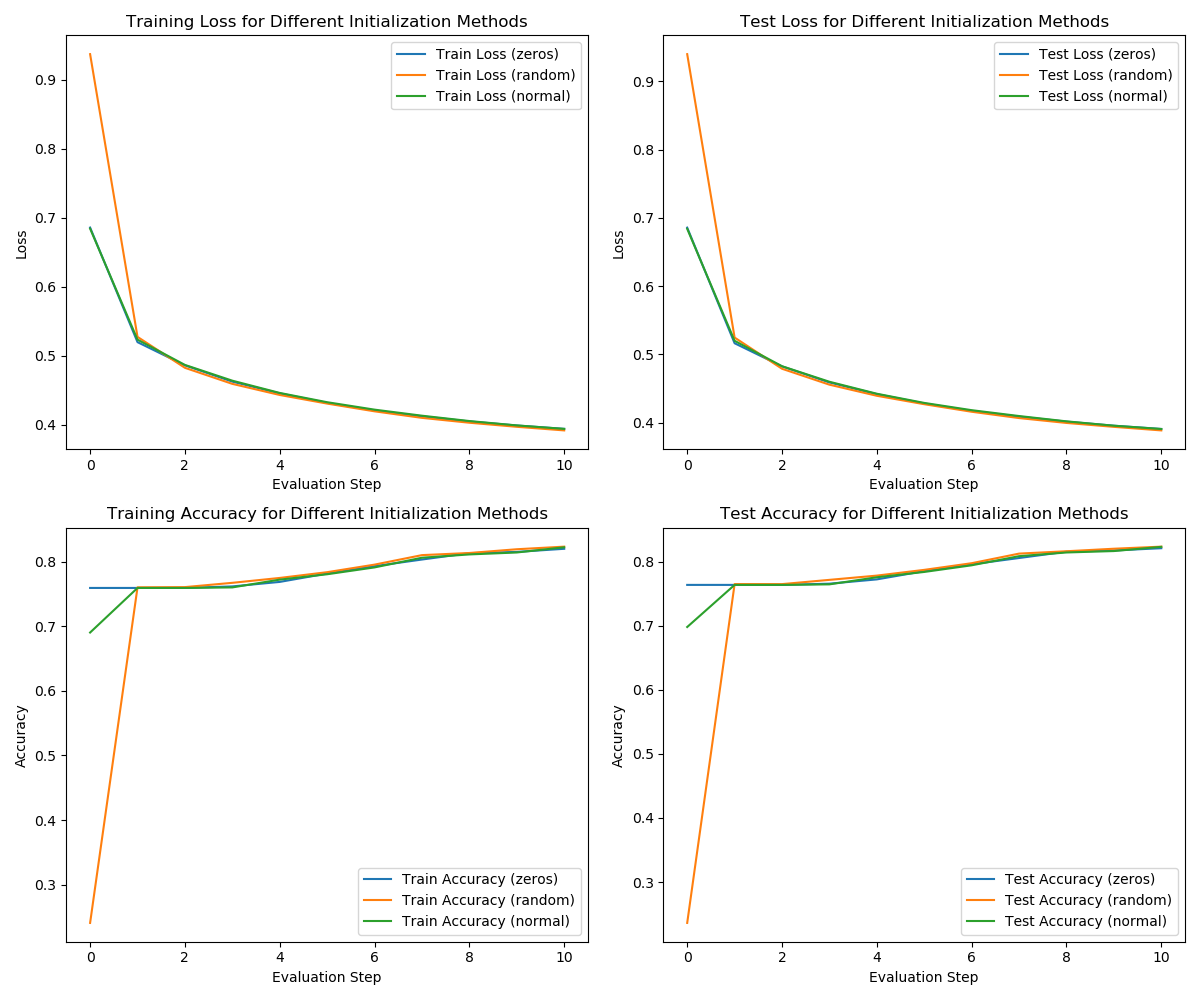
\includegraphics[width=\linewidth]{logistic_regression_init_methods.png}
\caption{逻辑回归不同初始化方法的比较。}
\label{fig:lr_init}
\end{figure}

图\ref{fig:lr_init}展示了不同初始化方法对逻辑回归性能的影响。虽然所有方法最终都会收敛,但正态和随机初始化相比零初始化达到更快的收敛速度。这是因为零初始化可能导致网络中的对称性,使所有神经元学习相同的特征。

\subsubsection{优化器比较}
\begin{figure}[htbp]
\centering
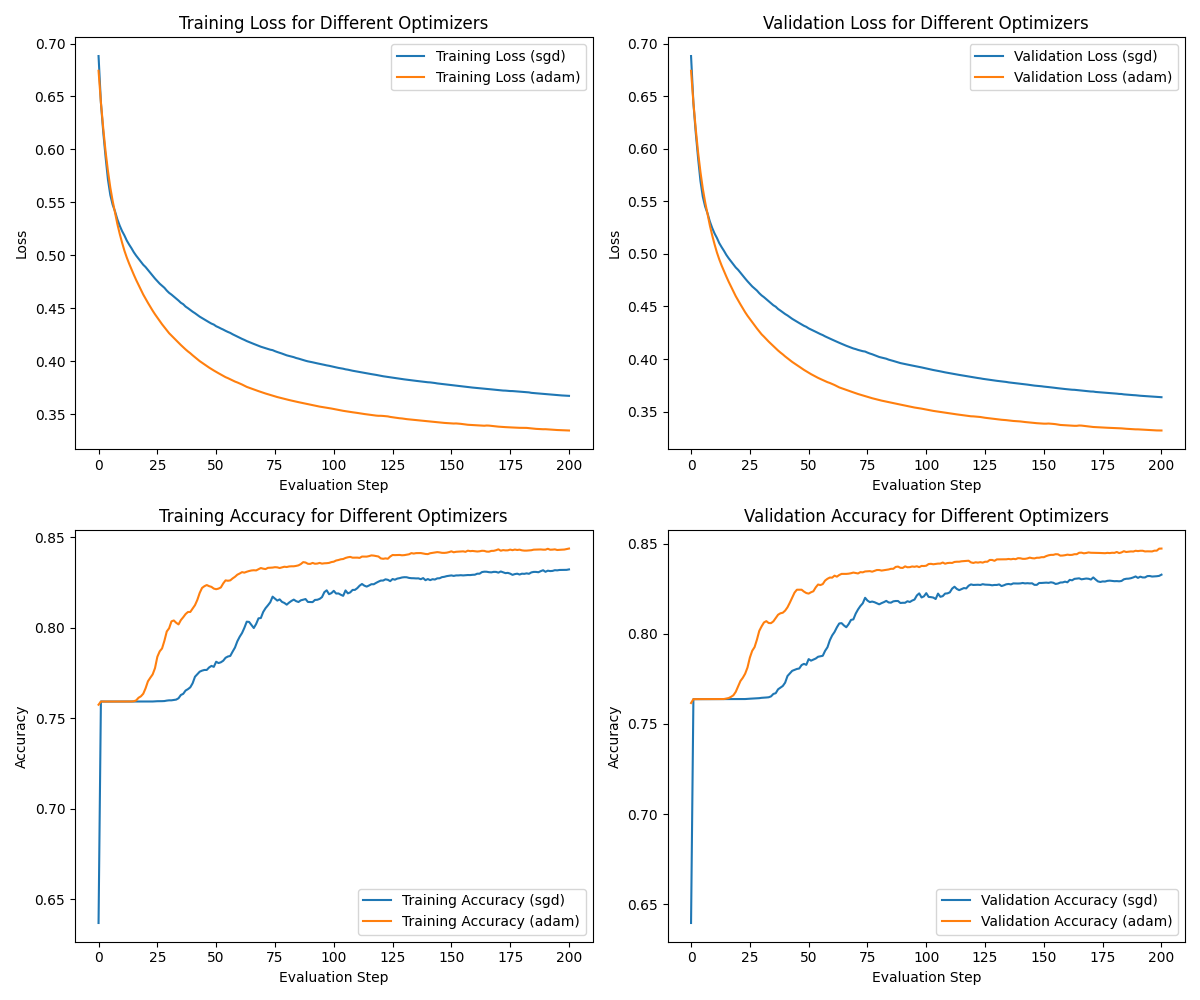
\includegraphics[width=\linewidth]{logistic_regression_optimizers.png}
\caption{逻辑回归中SGD和Adam优化器的性能比较。}
\label{fig:lr_opt}
\end{figure}

图\ref{fig:lr_opt}表明Adam优化器始终优于SGD,实现更快的收敛和更好的最终性能。这归因于Adam的自适应学习率和动量,有助于克服局部最小值和鞍点。

\subsubsection{批量大小的影响}
\begin{figure}[htbp]
\centering
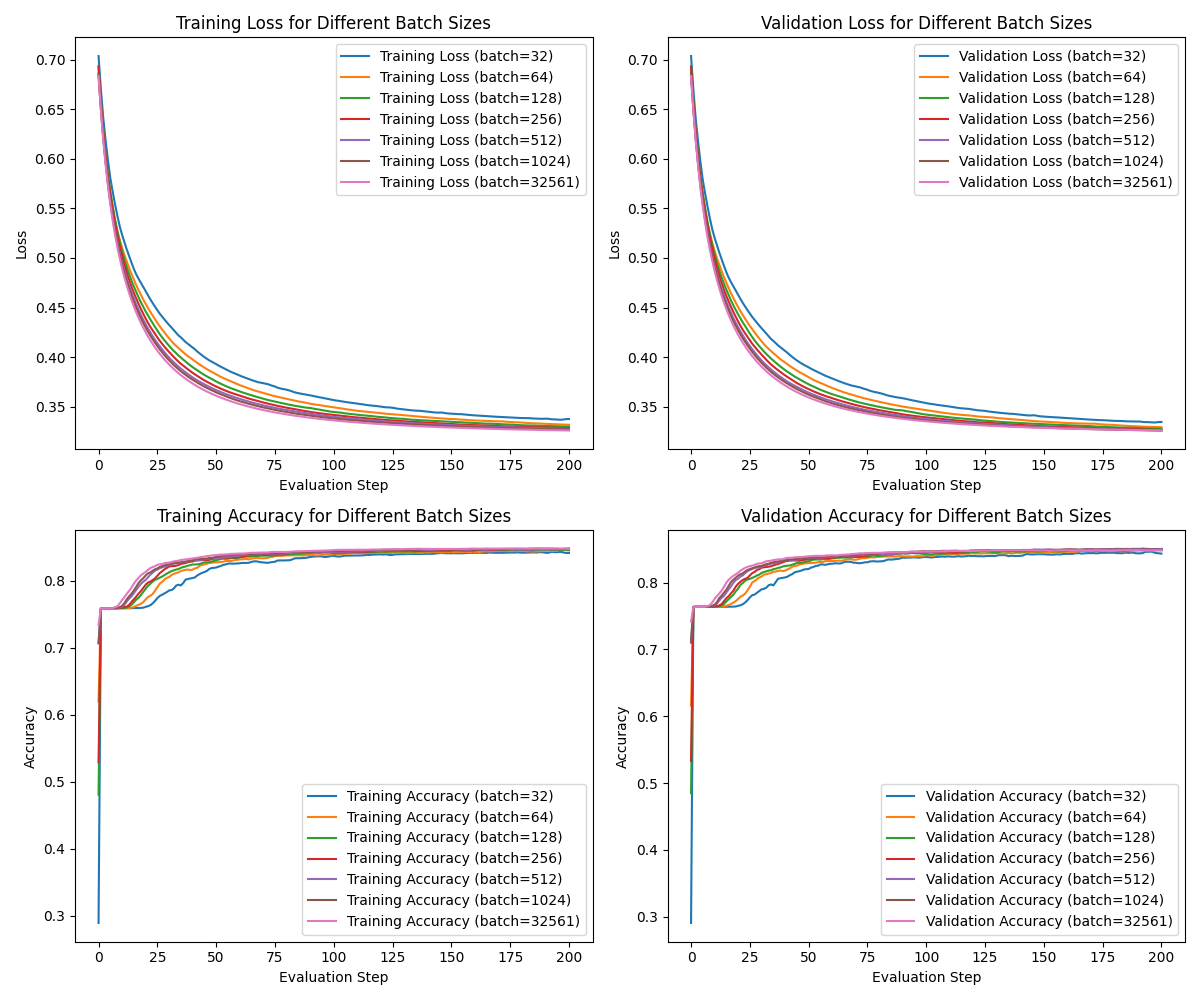
\includegraphics[width=\linewidth]{logistic_regression_batch_sizes.png}
\caption{不同批量大小对逻辑回归性能的影响。}
\label{fig:lr_batch}
\end{figure}

图\ref{fig:lr_batch}显示较小的批量大小(32)导致更嘈杂但可能更快的学习,而较大的批量大小(128)导致更平滑的收敛但可能陷入局部最优。中等批量大小(64)在收敛速度和稳定性之间提供了良好平衡。

\subsection{SVM结果}

\subsubsection{初始化方法的影响}
\begin{figure}[htbp]
\centering
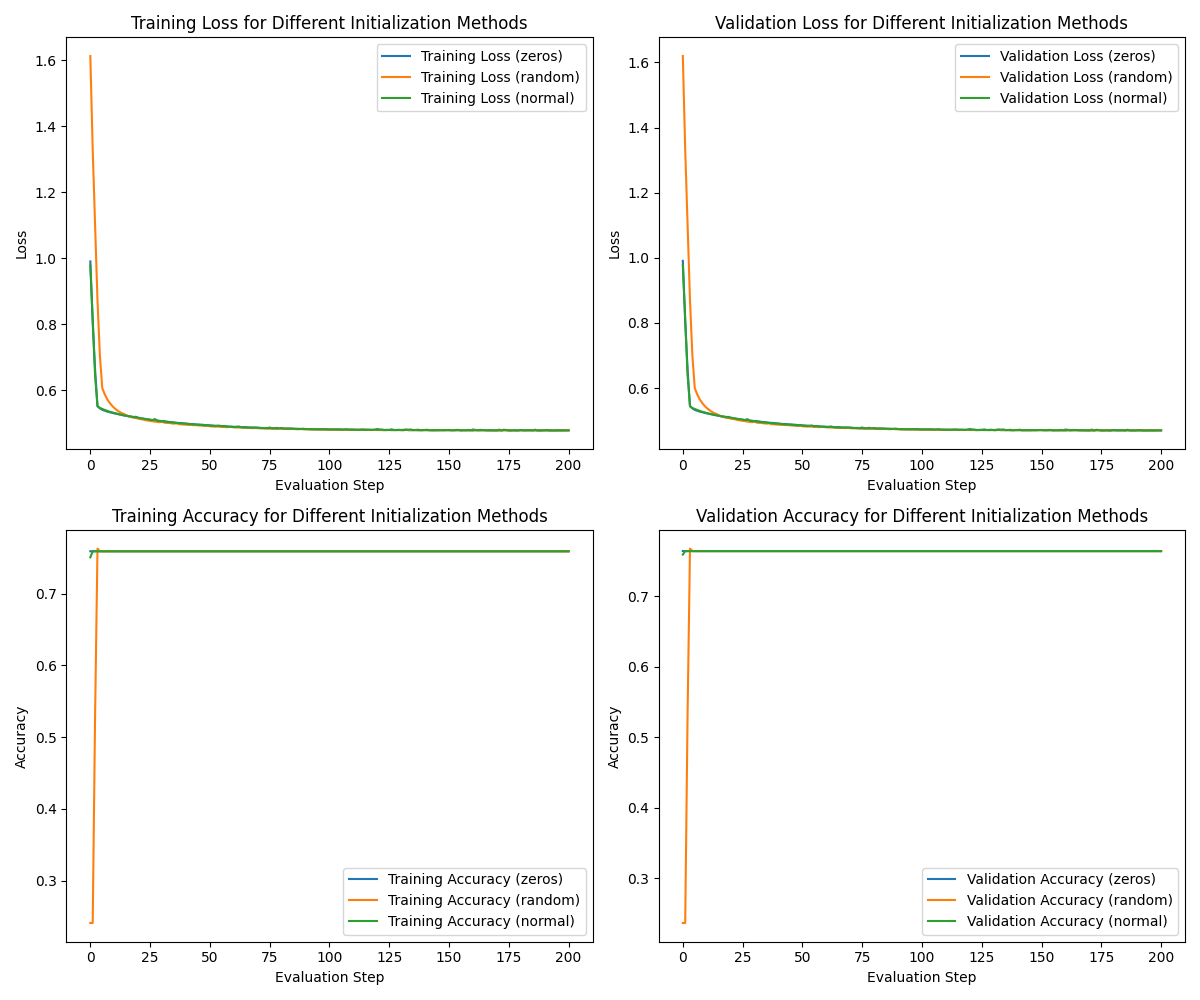
\includegraphics[width=\linewidth]{svm_init_methods.png}
\caption{SVM不同初始化方法的比较。}
\label{fig:svm_init}
\end{figure}

与逻辑回归类似,正态和随机初始化方法在SVM中表现优于零初始化,如图\ref{fig:svm_init}所示。然而,与逻辑回归相比,差异不太明显,表明SVM可能对初始化更加稳健。

\subsubsection{优化器比较}
\begin{figure}[htbp]
\centering
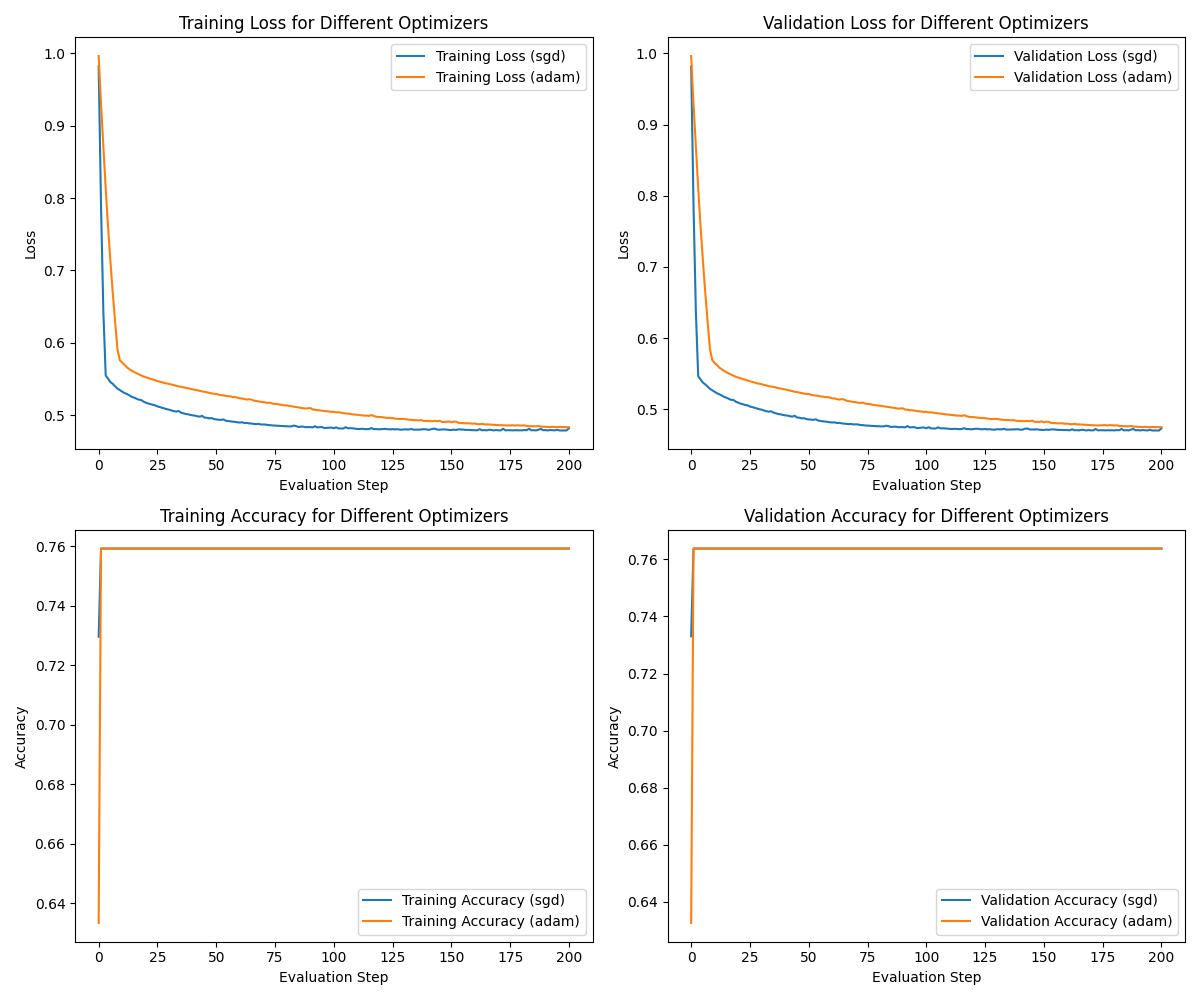
\includegraphics[width=\linewidth]{svm_optimizers.png}
\caption{SVM中SGD和Adam优化器的性能比较。}
\label{fig:svm_opt}
\end{figure}

图\ref{fig:svm_opt}确认Adam优化器在SVM中也优于SGD。Adam的自适应学习率有助于更有效地应对铰链损失函数的非平滑性质。

\subsubsection{损失函数比较}
\begin{figure}[htbp]
\centering
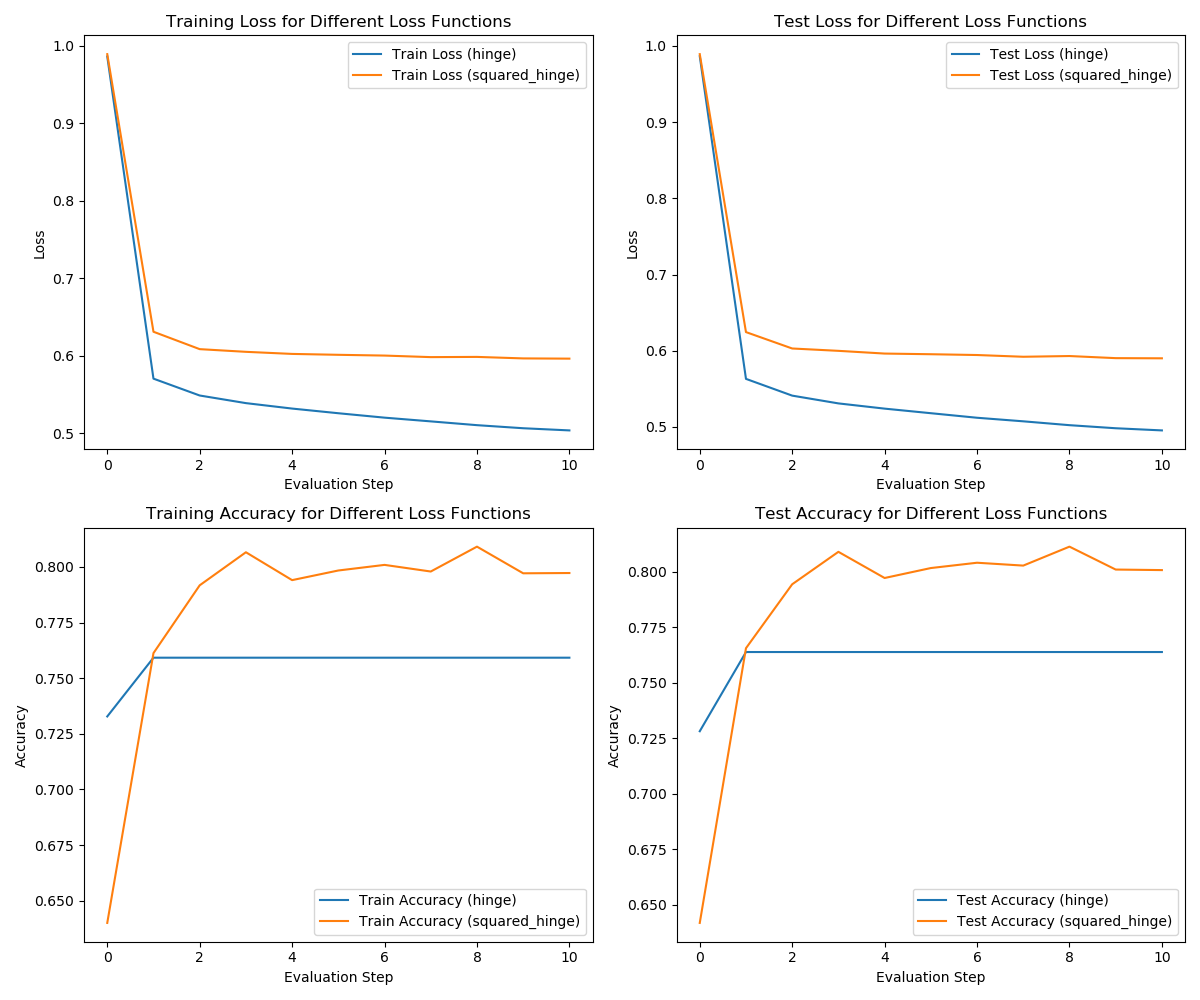
\includegraphics[width=\linewidth]{svm_loss_functions.png}
\caption{SVM中铰链损失和平方铰链损失的性能比较。}
\label{fig:svm_loss}
\end{figure}

图\ref{fig:svm_loss}比较了铰链损失和平方铰链损失。平方铰链损失由于对违规惩罚更强而显示出更快的收敛速度,但标准铰链损失在测试集上展示出略好的泛化能力。

\subsection{逻辑回归与SVM比较}

\begin{figure}[htbp]
\centering
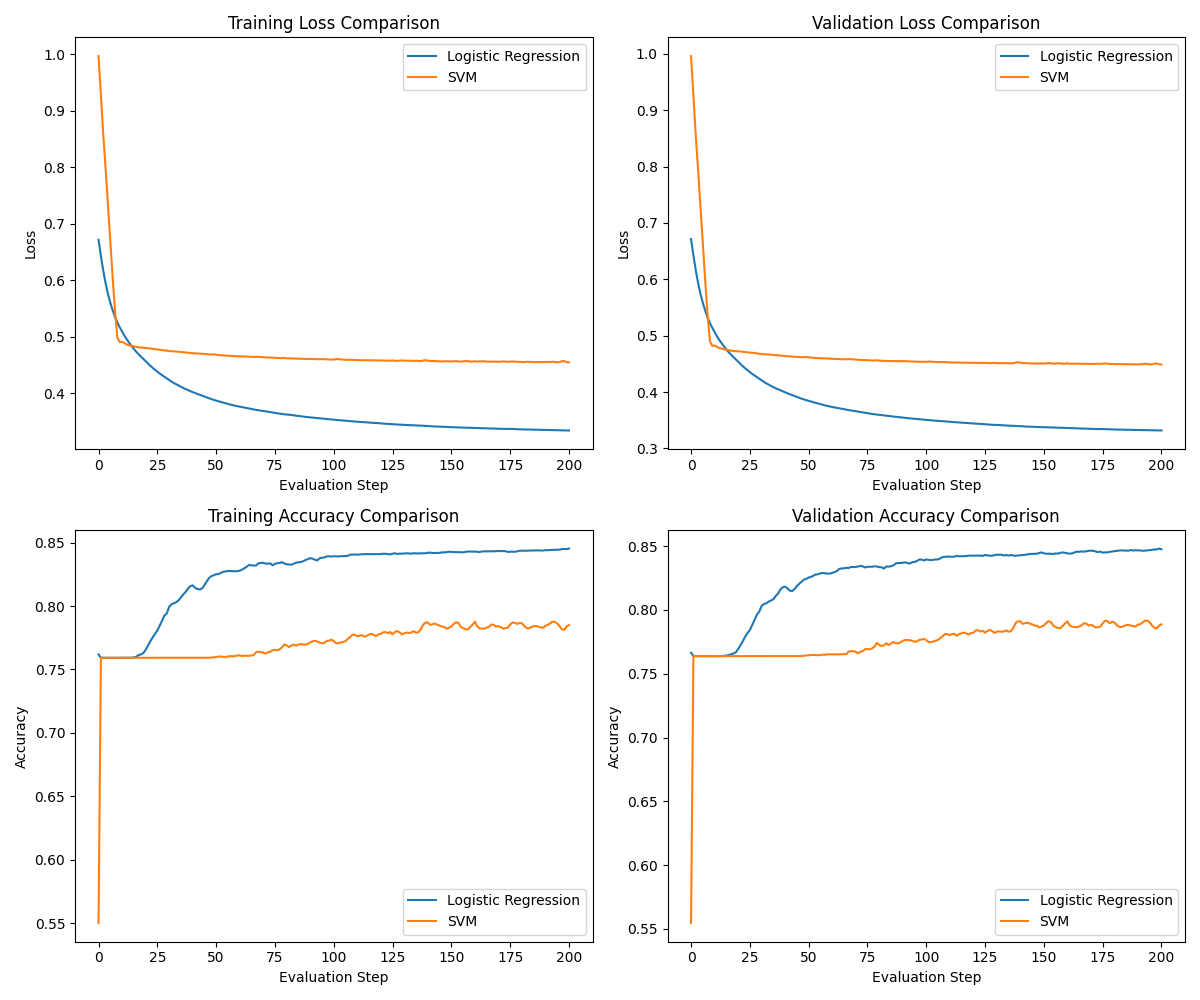
\includegraphics[width=\linewidth]{lr_vs_svm_comparison.png}
\caption{逻辑回归与SVM的性能比较。}
\label{fig:lr_vs_svm}
\end{figure}

图\ref{fig:lr_vs_svm}比较了逻辑回归和SVM的最佳配置。两种模型在测试集上达到相似的准确率,但它们显示出不同的训练特征:

\begin{table}[htbp]
\centering
\caption{逻辑回归与SVM的性能比较}
\label{tab:comparison}
\begin{tabular}{lcccc}
\toprule
\textbf{模型} & \textbf{准确率} & \textbf{精确率} & \textbf{召回率} & \textbf{F1分数} \\
\midrule
逻辑回归 & 0.8401 & 0.7321 & 0.5094 & 0.6007 \\
SVM & 0.8399 & 0.6988 & 0.5666 & 0.6258 \\
\bottomrule
\end{tabular}
\end{table}

表\ref{tab:comparison}显示SVM在所有指标上略微优于逻辑回归。这可归因于SVM的间隔最大化特性,通常导致更好的泛化,特别是在高维空间中。

\section{讨论}

\subsection{梯度下降与随机梯度下降}
我们的实验证明了随机梯度下降(SGD)相比全批量梯度下降的有效性。通过使用小批量,SGD提供了几个优势:

\begin{itemize}
    \item 由于参数更新更频繁,收敛更快
    \item 由于一次只处理数据的一个子集,内存需求减少
    \item 通过采样中固有的噪声实现更好的泛化,有助于摆脱局部最小值
\end{itemize}

最佳批量大小取决于具体问题,但我们的实验表明,中等批量大小(32-64)通常在计算效率和收敛稳定性之间提供良好平衡。

\subsection{逻辑回归与SVM}
虽然两种算法都旨在找到线性决策边界,但它们在优化目标上有所不同:

\begin{itemize}
    \item 逻辑回归最小化对数损失,专注于正确建模类别成员概率
    \item SVM最大化类别间间隔,专注于找到最稳健的决策边界
\end{itemize}

我们的结果表明,SVM在分类指标方面略微优于逻辑回归。这与理论一致,因为SVM的间隔最大化方法通常导致更好的泛化,特别是在有限训练数据的高维空间中。

然而,逻辑回归提供概率估计,这在需要风险评估或置信度分数的应用中很有价值。此外,逻辑回归可以更容易地扩展到多类问题,而不需要多个二分类器。

\subsection{优化方法}
我们对SGD和Adam优化器的比较一致表明,Adam在收敛速度和最终性能方面优越。Adam结合了以下几个优势:

\begin{itemize}
    \item AdaGrad,根据历史梯度调整学习率
    \item RMSProp,使用平方梯度的移动平均
    \item 动量,在相关方向上加速收敛
\end{itemize}

这种组合使Adam对非凸优化问题(如神经网络)特别有效,但我们的实验表明,它也有利于像逻辑回归和SVM这样的经典算法。

\section{结论}
在本实验中,我们从头实现并比较了逻辑回归和SVM算法。我们在a9a数据集上的实验提供了以下关键见解:

\begin{itemize}
    \item 参数初始化显著影响收敛速度,随机和正态初始化优于零初始化
    \item Adam优化器在逻辑回归和SVM中始终优于SGD
    \item 较小的批量大小导致更快但更嘈杂的学习,而较大批量提供更稳定但可能更慢的收敛
    \item 使用铰链损失的SVM在分类指标方面略微优于逻辑回归,证实了其在泛化方面的理论优势
\end{itemize}

这些发现深化了我们对逻辑回归和使用SVM的线性分类之间联系和差异的理解,以及不同优化策略对模型性能的影响。

未来工作可以探索核方法以扩展SVM到非线性可分问题、这些算法的多类扩展以及更复杂的正则化技术,以进一步提高泛化能力。

\begin{thebibliography}{00}
\bibitem{bishop} C.M. Bishop, "Pattern Recognition and Machine Learning," Springer, 2006.
\bibitem{vapnik} V. Vapnik, "The Nature of Statistical Learning Theory," Springer, 1995.
\bibitem{bottou} L. Bottou, "Large-Scale Machine Learning with Stochastic Gradient Descent," Proceedings of COMPSTAT'2010, pp. 177-186, 2010.
\bibitem{kingma} D.P. Kingma and J. Ba, "Adam: A Method for Stochastic Optimization," International Conference on Learning Representations, 2015.
\end{thebibliography}

\end{CJK}
\end{document} 